\documentclass[a4paper,10pt]{scrartcl}
%encodings
\usepackage[utf8]{inputenc}
\usepackage[english]{babel}
\usepackage[T1]{fontenc}
%colors, hyperrefs
\usepackage{color}
\usepackage{url}
\usepackage[pdftex,pdfauthor={J\"org Behrmann, Anika Haller},pdftitle={Ma2: Low Energy Electron Diffraction (LEED)}]{hyperref}
%figures and subfigures
\usepackage[pdftex]{graphicx}
\usepackage{subfigure}
%better tables
\usepackage{tabularx}
\usepackage{booktabs}
\usepackage{multirow}
%math stuff
\usepackage{amsmath}
\usepackage{amsthm}
\usepackage{amsfonts}
\usepackage{IEEEtrantools}
\usepackage[square,comma,numbers,sort&compress]{natbib}
%shiny stuff
\usepackage[babel]{microtype}
\DisableLigatures{encoding=T1,family=tt*}

\usepackage{textcomp}

\begin{document}

\title{Low Energy Electron Diffraction (LEED)}
\author{J\"org Behrmann\footnote{behrmann@physik.fu-berlin.de} \qquad Anika Haller\footnote{halleran@zedat.fu-berlin.de}}
\date{21.11.2011}
\maketitle
\tableofcontents
\thispagestyle{empty}

\section{Introduction}

In 1924 Louis de Broglie proposed the Particle Wave duality implying that particles could have wave-like characteristics. This was proofed in 1926 by Davisson and Germer, who used the wave-properties of electrons to study Ni crystals. 

Their work is ancestral to the Low Energy Electron Diffraction, which is a spectroscopic technique that is used to study crystal surfaces and substrates on surfaces. LEED came up in the 1960s because of the need ultra high vacuum (UHV) that is needed. Electrons are favorable for surface structure analysis because they are easier to produce than neutrons and are much more sensitive to surfaces than X-rays because of their very short mean free path in solids.

\subsection{Particle Wave Duality}

The wavelength of a particle is given by the de Broglie relation
\begin{equation}
\lambda = \frac{h}{p} = \frac{h}{\sqrt{2mE_{kin}}} \label{eq:broglie1}
\end{equation}
where h is Planck's constant. For an charged particle that is accelerated by the voltage $U$ this amounts numerically to
\begin{equation}
\lambda = 12.26 \mbox{\AA} \sqrt{\frac{\mbox{ev}}{E_{kin}}} = 12.26 \mbox{\AA} \sqrt{\frac{\mbox{eV}}{qE}} \label{eq:broglie}
\end{equation}
When the wavelength of a particle is approximately equal to the lattice constant it can be used to examine the surface. For acceleration voltages in the range between $50$ to $500\,$V an electron's wavelength will be between $0.5$ and $2\,$\AA. Relativistic corrections are not needed at this energies, because 
\begin{equation}
\frac{E_{kin}}{E_0}=\frac{eU}{mc^2} \approx 1\mbox{\textperthousand}
\end{equation}

\subsection{Diffraction}

\subsection{Far Field Approximation}

When a plane wave $Ae^{ikx}$ falls on a pointlike scatterer it becomes the source of radial waves of the form
\begin{equation}
\phi=\int dy J(y)\frac{e^{i|k||x-y|}}{|x-y|} A e^{iky}, \label{eq:scatter}
\end{equation}
where the integration is over the whole scatterer and $J(x)$ describes the the response of the medium. The above expression can be found by finding the Green's function to the wave equation.
\begin{equation}
\phi(x)=\frac{A}{R}e^{ik'x}\int dyJ(y)e^{i(k-k')y}  \label{eq:farfield}
\end{equation}
This formula is~\eqref{eq:scatter} in the far field approximation, i.e. far away from the scattering event, which is most certainly true for our experiment. Additionally we assumed that the incoming wave is not substantially altered by the scattering event. In quantum mechanics this is called the Born approximation; it neglects subsequent scattering, because they are of order $J^{2}(x)$, as is known from basic courses on scattering theory. This assumption is save if $J(x)$ is much smaller than one, i.e. weak scattering potentials.

Equation~\eqref{eq:farfield} tells us that what can be experimentally observed is basically the Fourier transform of the scattering potential. 

\subsection{The Reciprocal lattice, Laue condition and Bragg formula}

We will now assume a form for $J(x)$
\begin{equation}
J_{A}(x)=\sum_{r\in\mathbb{\mathbb{Z^{n}}}}\delta(x-A\cdot r) \label{eq:dirac}
\end{equation} 
where $A$ is the $n \times n$ matrix of unit vectors of the lattice and x and r are n-dimensional vectors in the lattice. Equation~\eqref{eq:dirac} is the n-dimensional Dirac lattice, which for example for $n=1$ is called a Dirac comb. 

A well-known theorem on Fourier transformation tells us that the Fourier transform of a lattice is again a lattice
\begin{equation}
J(k)=\sum_{g\in\mathbb{Z}^{n}}\delta(k-G \cdot g),\quad \mbox{with} \quad G=2\pi(A^{-1})^{T}=2\pi A^{-T}. \label{eq:recproc}
\end{equation}
$G$ is the so-called reciprocal lattice and $g$ are the reciprocal lattice vectors. We now need to identify $k$ in~\eqref{eq:recproc} with $k-k'$ in equation~\eqref{eq:farfield}. This gives us the Laue condition, which states that we observe a peak whenever $k-k'$ equals a reciprocal lattice vector. This can be visualized quite nicely with the Ewald construction that can be found in figure~\ref{fig:ewald}.

\begin{figure}
\centering
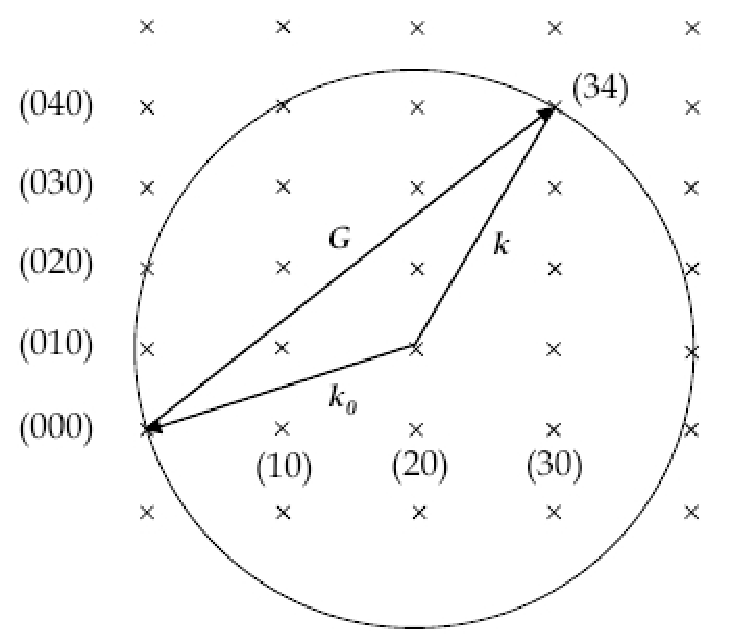
\includegraphics[scale=0.45]{img/ewald}
\caption{Ewald construction for the Laue condition. \label{fig:ewald}}
\end{figure}

The Laue condition is equivalent to the Bragg formula, which can be seen by squaring.
\begin{eqnarray}
g^{2} & = & k^{2}-2kk'+k'^{2} \\  
g^{2} & = & 2k^{2} (1-\cos \alpha) \\
g^{2} & = & 4k^{2}\sin^{2}\theta \label{eq:prebragg}
\end{eqnarray}
where $\alpha = 2 \theta$ is the angle between $k$ and $k'$. From the definition of the reciprocal lattice we can see that each reciprocal lattice vector is associated with a family of planes whose distance is given by $d=\tfrac{2\pi n}{|g|}$, where $n$ is a natural number so that $\tfrac{g}{n}$ is still a reciprocal lattice vector. Inserting this in the above equation we arrive at the Bragg formula
\begin{equation}
\lambda=2nd\sin\theta. \label{eq:bragg}
\end{equation}

In reality lattices will not be delta lattices. One will then need to add a structure factor to model the internal structure of a unit cell. Also peaks are not infinitely sharp delta peaks, so that a factor---the finite size factor---is needed to give them a finite width.

\subsubsection{A Two-Dimensional Lattice}

In the two-dimensional case the lattice matrix is given by 
\begin{equation}
A=\left(\begin{array}{cc}
a & 0\\
0 & a
\end{array}\right) \Longleftrightarrow G=\frac{2\pi}{a}\left(\begin{array}{cc}
1 & 0\\
0 & 1
\end{array}\right). 
\end{equation}
The scattering potential is then given by 
\begin{equation}
J(k)=\sum_{n,m}\delta(k-G \cdot g) \quad \mbox{with} \quad k=\left(\begin{array}{cc}
k_{x} \\
k_{y}
\end{array}\right)\mbox{,}~g=\left(\begin{array}{cc}
m \\
n
\end{array}\right)
\end{equation}
Inserting $g$ in equation~\eqref{eq:prebragg} we arrive at the according formula for the two-dimensional case.
\begin{equation}
\sin\theta_{nm}=\frac{\lambda}{a}\sqrt{m^{2}+n^{2}} \label{eq:bragg2}
\end{equation}

In our experiment we will examine a copper surface using formula~\eqref{eq:bragg2}. Copper has a lattice constant of $a=2.55\,$\AA and our analyzer has can be fixed at angles of $45$\textdegree and $52$\textdegree. Using equation~\eqref{eq:broglie} together with equation~\eqref{eq:bragg2} one arrives at
\begin{equation}
\frac{E_{kin}}{\mbox{eV}} = \frac{(12.26\,\mbox{\AA})^{2}}{a^2 \sin\theta}  (m^2 + n^2)
\end{equation}
which we used to calculate the needed energies that can be found in table~\ref{tab:reqenerg}. The appropriate diffraction patterns can be found in figure~\ref{fig:reflexes}

\begin{figure}
\centering
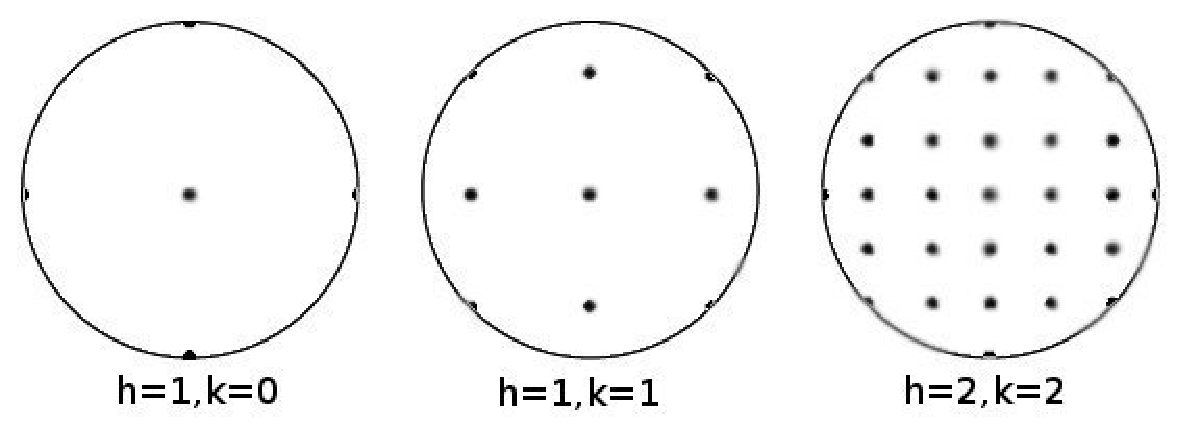
\includegraphics[scale=0.4]{img/reflexes}
\caption{Expected diffraction patterns for different energies \label{fig:reflexes}}
\end{figure}

\begin{table}
\begin{center}
\begin{tabular}{lcc}
\toprule
Reflex  & Energy\mbox{\,}[eV] at $\theta=45$\textdegree & Energy\mbox{\,}[eV] at $\theta=52$\textdegree \\
\midrule
(0,1) & \phantom{0}46.23 & \phantom{0}37.22 \\
(1,1) & \phantom{0}92.46 & \phantom{0}74.45 \\
(2,2) & 369.84 & 297.80 \\
\bottomrule
\end{tabular}
\end{center}
\par
\caption{Required electron energies for certain reflexes \label{tab:reqenerg}}
\end{table}

\subsection{Superstructures}

In our experiment we will adsorb oxygen O$_2$ on the copper surface we will examine. The oxygen will form a regular lattice structure on top of the copper surface---a so-called ($\sqrt{2} \times 2\sqrt{2}$)R$45$\textdegree superstructure. This superstructure notation, due to Woods, means that the lattice of the superstructure is obtained by scaling the x-direction by a factor of $\sqrt{2}$ and the y-direction by a factor of $2\sqrt{2}$ and rotating the lattice then by $45$\textdegree.

The superstructure will change the reciprocal lattice constants accordingly: $\tfrac{2\pi}{\sqrt{2}a}$  in the x- and $\tfrac{2\pi}{2\sqrt{2}a}$ y-direction.

The superstructure will also introduce a structure factor, since the unit cell is not now more complicated, which will make the former copper peaks stronger. 

\begin{figure}
\centering
\subfigure[ ]{
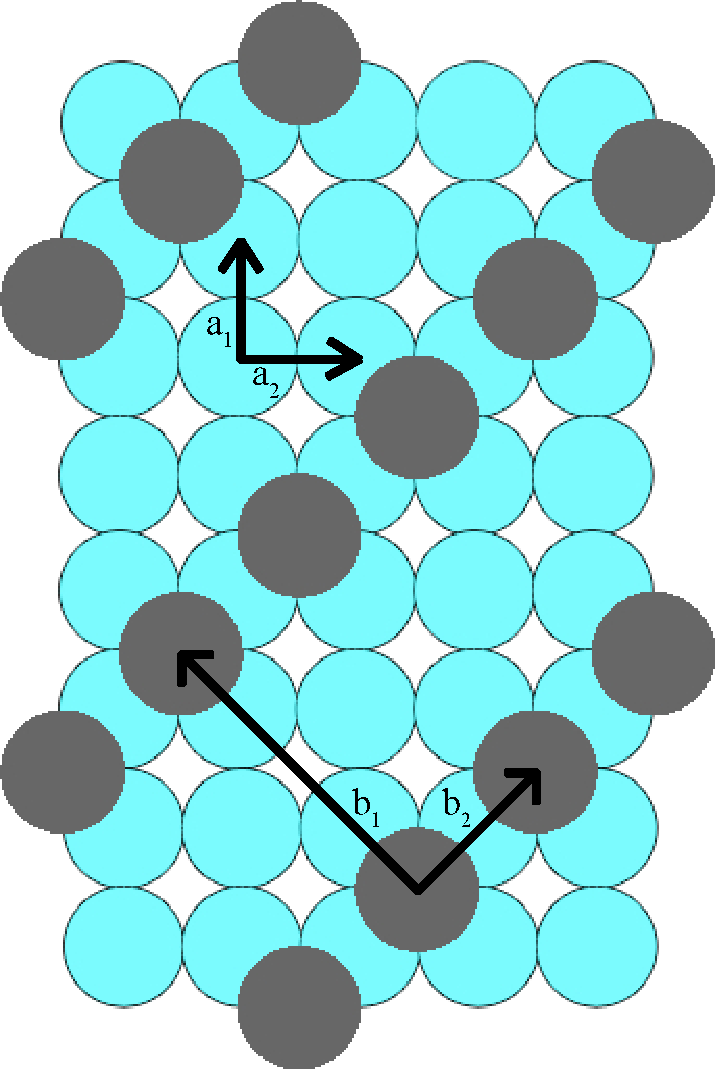
\includegraphics[scale=0.25]{img/superstructure1}
\label{fig:sup1}
}
\subfigure[ ]{
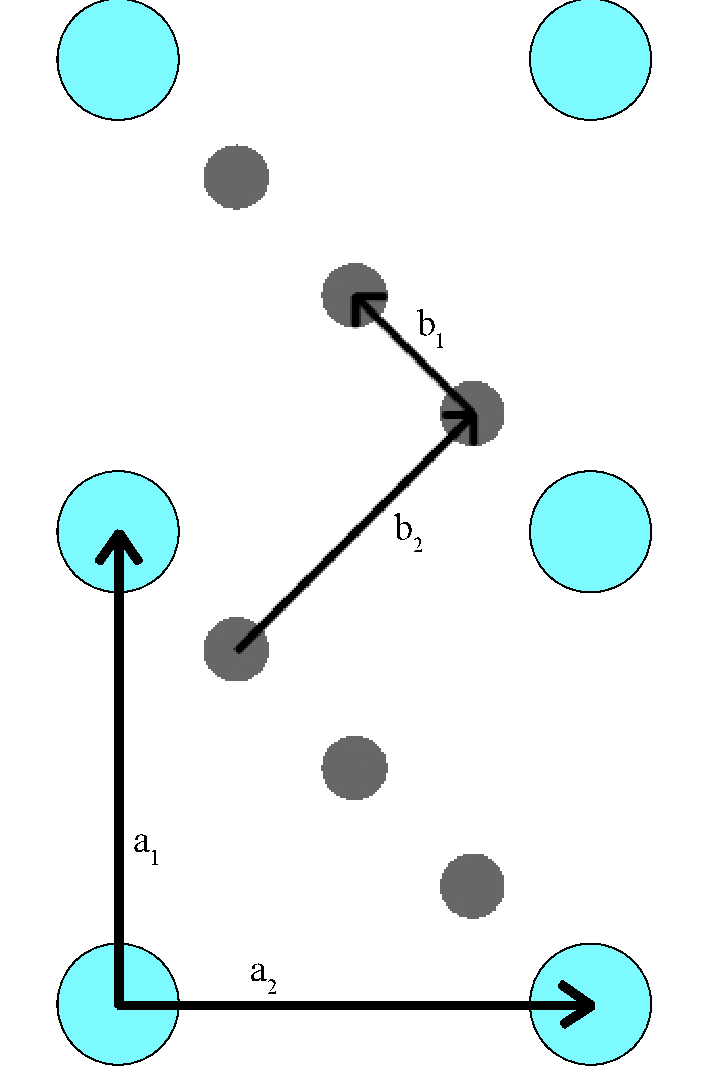
\includegraphics[scale=0.25]{img/superstructure2}
\label{fig:sup2}
}
\subfigure[ ]{
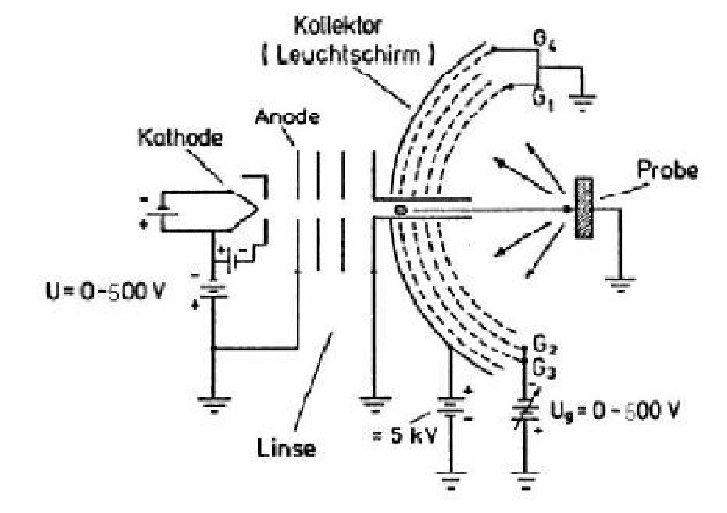
\includegraphics[scale=0.45]{img/setup}
\label{fig:setup}
}
\caption{The blue lattice in \subref{fig:sup1} is the regular lattice with lattice vectors $a_i$ and the gray lattice shows the ($\sqrt{2} \times \sqrt{2}$)R$45$\textdegree superstructure with lattice vectors $b_i$, \subref{fig:sup2} shows the same lattice in reciprocal space. \subref{fig:setup} shows the experimental setup.}
\end{figure}

\subsection{Kinematic Approximation}

LEED can also be used to investigate the perpendicular lattice constant. Since the electrons need to penetrate the first lattice layer of the lattice and enter a strong potential, the simple model excluding multiple scattering events needs to be modified. We first modify equation~\eqref{eq:broglie1}
\begin{equation}
\lambda = \frac{h}{p} = \frac{h}{\sqrt{2m(E_{kin}-V)}}
\end{equation}
to account for energy loss in the scattering events. We will approximate $V$ as a constant potential. Using the above redefinition the perpendicular lattice constant is given by
\begin{equation}
2a_{\perp} = n\lambda = n \sqrt{\frac{h^{2}}{2m(E_{kin}-V)}}.
\end{equation}

\section{Experimental Setup}

\subsection{LEED apparatus}

The LEED apparatus consists of a vacuum chamber in which an electron gun is situated that produces electrons by thermoemission, shapes a beam and accelerates towards a target, which is located on a moveable arm. The vacuum is maintained by pumps described below. To direct the beam two copper coils are wound around the vacuum chamber to cancel the earth's magnetic field. To clean the sample a sputtering gun is mounted inside the vacuum chamber. The sputtering gun works by accelerating inert ions twoards the sample. Inert ions have to be used, so that they do not react with or adsorb to the sample.

The electrons hitting the sample are diffracted and fall on a spherical screen, where they are made visible by flourescence. Inelastically scattered electrons are suppressed using a suppression grid and the contrast of the screen can be manipulated by another acceleration grid. The peaks appearing in the screen are taken using a CCD camera, which can be controlled externally by a computer, as can be the electron gun.

A schematic of the LEED apparatus is shown in figure~\ref{fig:setup}.

\subsection{Ultra-High Vacuum (UHV)}

The current experiment will be done in UHV, because of the very short mean free path of electrons in matter. The vacuum will be obtained by using a cascade of pumps to obtain ever lower pressures.  The first pump used is a \textit{rotary vane pump}, which is a simple mechanical pump that is basically a rotating cylinder with attached vanes shoveling out the gas, thus producing a prevacuum. The next step is a \textit{turbomolecular pump}, which works in the prevacuum by rotating a fan consisting of several blades at the speed of the remaining gas molecules. The blades hit the gas molecules kicking them out of the chamber. 

Even higher vacuums can be obtained by using absorption pumps, in our case an \textit{ion getter pump} and an \textit{titan sublimation pump}. The ion getter pump works by ionizing remaining gas atoms through an electron beam and pulling them out with an electric field. Applying an additional magnetic field improves this pump, since the ions move on orbits in the magnetic field, ionizing more gas atoms on their way. The titan sublimation pump works by binding remaining gas molecules chemically through the use of a reactive element, in our case titanium. This last pump is only used in between experiments so as to not contaminate the sample.

\section{Experimental Procedure}

\subsection{Preliminary Procedures}

To clean the copper sample from the remainings of the previous group the sample was sputtered by switching off the ion getter pump and opening the the Argon valve thus increasing the pressure in the LEED chamber to about $5 \cdot 10^{-5}\,$mbar. The sample was sputtered for 35 minutes using Filament 1 with a beam voltage of $1.5\,$kV and an emission current of $20\,$mA. The ion getter pump was then restarted and the sample annealed for 20 minutes up to a temperature of 535 degrees centigrade o restore the copper surface. After that the sample was allowed to cool off for an hour until the pressure in the LEED chamber normalized to about $9 \cdot 10^{-10}\,$mbar and the sample temperature fell to about 80 degrees centigrade. We then moved on to calibrate the LEED apparatus setting the fluorescence voltage to $6\,$kV, the upper power supply for the magnets to $2.65\,$A and $0.07\,$V and the lower power supply to $2.80\,$A and $0.13\,$V.

\subsection{Lattice constant measurements}

After calibration of the LEED apparatus we controlled the power supply and CCD camera of the apparatus from the external computer and took several series of LEED diffraction images in the energy range between $50$ and $300\,$eV in steps of $1\,$eV and saved them as avi-files, to later determine the lateral lattice constant.

For the determination of the perpendicular lattice constant we took an intensity-energy spectrum of the (0,0)-peak in the energy range between $40$ and $600\,$eV. To successfully do this part of the experiment the reflection of the electron gun had to be placed behind the electron gun itself so that the (0,0)-pea was visible between the electron gun and its cables on the left-hand-side and the aperture of the CCD camera had to be almost closed; otherwise the reflection of electron gun would outshine the (0,0)-peak.

\subsection{Adsorption of oxygen}

To absorb the oxygen on the surface the sample was preheated to about 300 degrees centigrade by applying a heating current of $3\,$A, that we later increased to $3.4\,$A, at $5.8\,$V to the sample for 10 minutes. This was done as to not burn the filament, while introducing oxygen into the chamber. We then opened the oxygen valve, increasing the pressure in the LEED chamber to $2 \cdot 10^{-6}\,$mbar. Noticing a rapid cooling of the sample we increased the pressure to $5.1 \cdot 10^{-6}\,$mbar two minutes later. About 10 minutes later we noticed, that we had forgotten to switch off the ion getter pump, he pressure fell rapidly to $1.2 \cdot 10^{-6}\,$mbar which we again regulated to $5 \cdot 10^{-6}\,$mbar. Ten minutes later we closed the oxygen valve an reevacuated the chamber. We then took energy scans as in the previous task in the energy range between $40$ and $300\,$eV in steps of $1\,$eV.

\section{Evaluation of Experimental Data}

To evaluate our experimental data we followed the method described by Tarasinski and Wölms~\cite{brian}. We wanted to improve on this method by automatizing it. This was not possible for reasons described later on.

The animated scans were dumped using \textit{ffmpeg}. We then experimented with image recognition algorithms on these images . This show to be futile for two reasons. 

For one, the electron gun and the outer regions showed to be very interesting, at least for image recognition algorithms, leading to a vast number of points of interest in all images. 

An even bigger obstacle surfaced while looking at long series of images, since we---unfortunately---decided during the experiment to save the scans as .avi-files, not realizing that it is a compressed format. This lead to a problem of ``blockiness'' of later images, i.e. images of higher energies. The data was still usable, since the direct relation of frame number to electron energy was not touched, and human image recognition works far better than algorithmic image recognition, but the additional noise introduced by compression made automated image recognition impossible.

Tarasinski and Wölms were so kind as to provide us with their original program to mark peaks in images to obtain the pixel coordinates.

If not mentioned otherwise Gaussian error calculus is used.

\subsection{Calibration}

To obtain the conversion factor from peak position in pixels (measured from upper left corner) to angular position we took several images of the (0,0)-spot at different angles and fitted it to the function
\begin{equation}
p = A \sin( \theta - \theta_{0} ) + c = A \sin( 2\alpha - \theta_{0} ) + c, \label{eq:calibmodel}
\end{equation}
where $p$ is the position in pixels, $A$ is the angle to pixel conversion factor and $c$ is a constant offset. The fitted model is motivated by the geometry of the screen and in the second equality the reflection law $\theta=2\alpha$ was used. The fitted model can be seen in figure~\ref{fig:calib} and the fit parameters can be found in table~\ref{tab:calibdata}, with $A$ being the only relevant data.

We thought it could be problematic, that the fitted model~\eqref{eq:calibmodel} could seem unmotivated, since all our calibration data points are in the linear region of the the sine, but figure~\ref{fig:imgcalib} shows the diffraction pattern for one of the most extreme angles, only one value for a smaller angle could be obtained before the reflection of the electron gun vanished and with it the (0,0)-spot. 

We therefore also fitted a linear model, that lead to similar results, only seen in figure~\ref{fig:calib}, which we used as an a posteriori check for the model, we used to evaluate the data.

\begin{table}
\begin{center}
\begin{tabular}{lcc}
\toprule
$A$\,[px] & $\theta_{0}$\,[deg] & $c$\,[px] \\
\midrule
$-283 \pm 24$ & $115 \pm 25$  & $283 \pm 114$ \\
\bottomrule
\end{tabular}
\end{center}
\par
\caption{Fit parameters for calibration curve \label{tab:calibdata}}
\end{table}

\begin{figure}
\centering
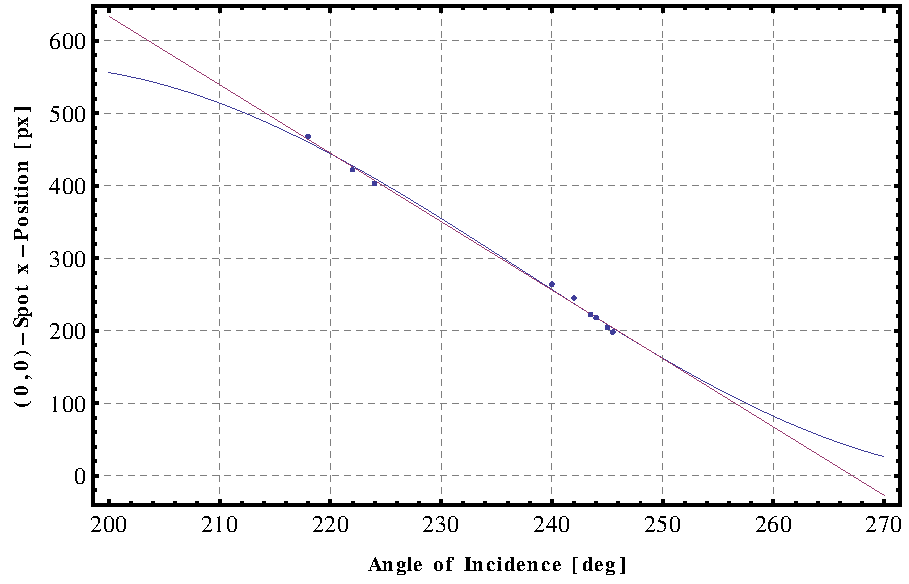
\includegraphics[scale=0.55]{img/calib}
\caption{Calibration curve \label{fig:calib}}
\end{figure}

\begin{figure}
\centering
\subfigure[ ]{
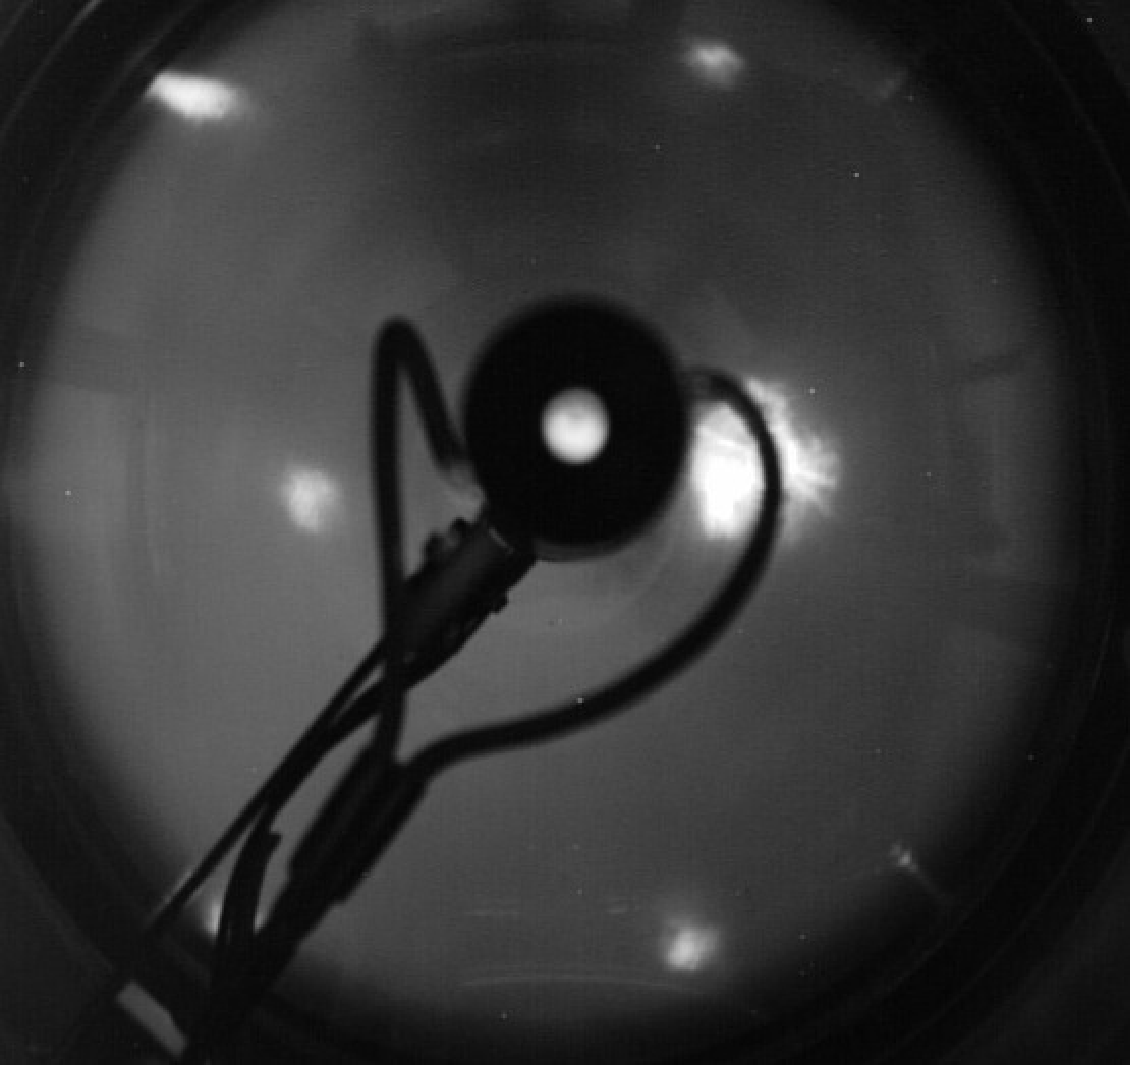
\includegraphics[scale=0.32]{img/calib_2220}
\label{fig:imgcalib}
}
\subfigure[ ]{
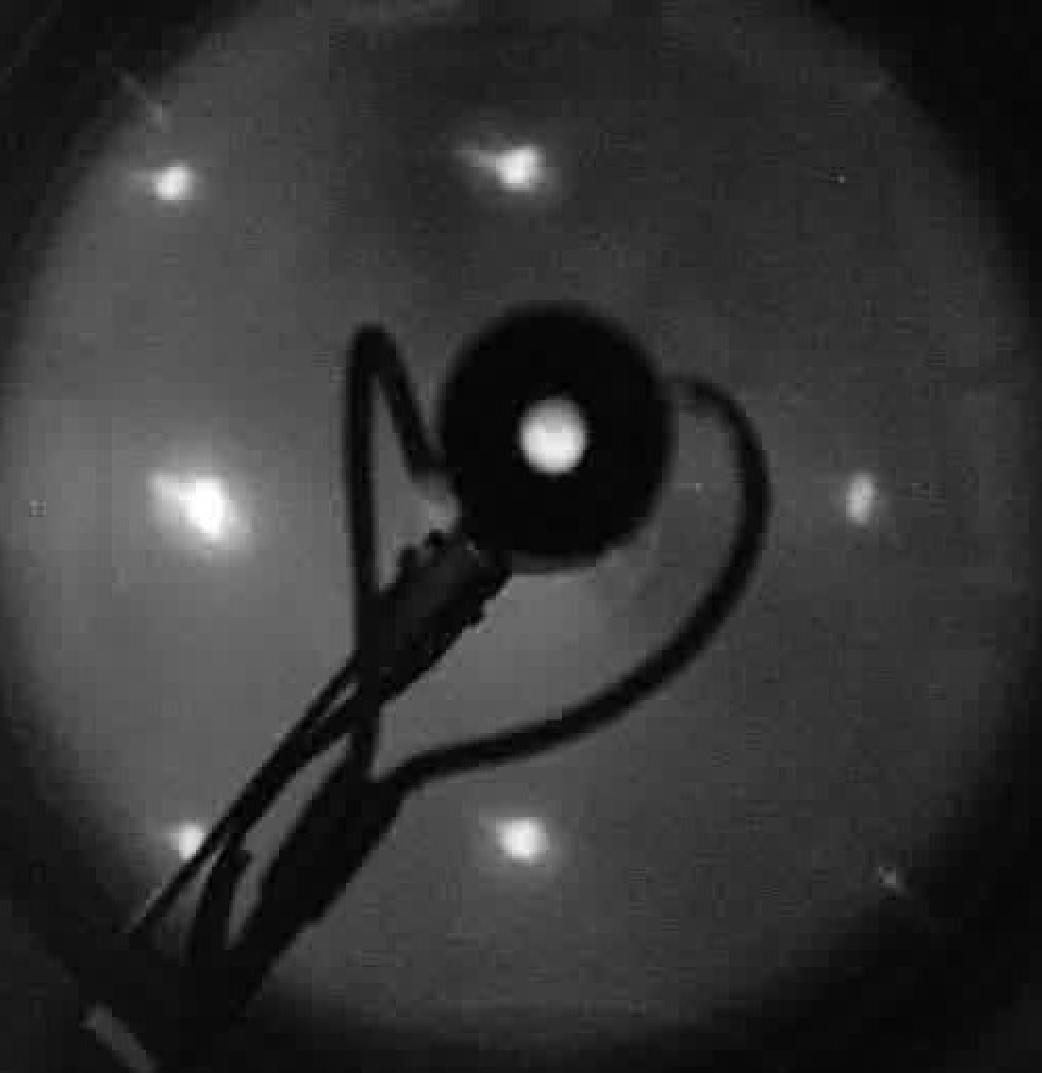
\includegraphics[scale=0.32]{img/img_scan_79ev}
\label{fig:imgscan}
}
\caption{ Figure~\subref{fig:imgcalib} shows an image from the calibration process, with the sample at $\theta = 222$\textdegree. The (0,0)-Peak can be seen as brighter spot in the lower left part of the big spot that is the reflection of the electron gun. Figure~\subref{fig:imgscan} shows an exemplary image (at $79\,$eV) from the scan to obtain the lateral lattice constant.}
\end{figure}


\subsection{Lateral Lattice Constant}

To calculate the lateral lattice constant we took a series of images of the LEED diffraction patterns in an energy range from $50$ to $300\,$eV with a step size of $1\,$eV. 

We then determined the pixel positions of all peak pairs (e.g. (1,0) and (-1,0)) over all images. These positions vary with electron energy. Not all peaks are visible for all energies, since some peaks only appear at higher energies, and all peak intensities also vary with energy. Additionally sometimes peaks vanish behind parts and cables of the electron gun and peaks on the right side of the screen are much fainter than only the left-hand side for a reason unknown to the authors.

From the recorded pixel positions of the peaks we then calculated the pixel distances $d$ for each peak pair, when both peaks of a pair were visible at a given energy. According to~\eqref{eq:calibmodel} $d/2$ for the peak pair (m,n) is directly proportional to the the sine of the scattering angle $\theta_{mn}$. Using~\eqref{eq:bragg2} we thus obtain
\begin{equation}
\frac{d}{2 A \sqrt{n^2 + m^2}} = \frac{d_{mn}}{2A} = \frac{\lambda}{a'}. \label{eq:latticemodel}
\end{equation}
A plot of~\eqref{eq:latticemodel} can be found in figure~\ref{fig:allscat}.

We then fitted the data in~\ref{fig:allscat} once as in~\eqref{eq:latticemodel} with a forced zero intercept, i.e. as a line through the origin, and once without forced zero intercept. The fit parameters for all peak pairs can be found in table~\ref{tab:calibdata}.

The errors for the fit parameters in table~\ref{tab:calibdata} are given purely from their distribution without explicit use of errors in their positions. Of course all positions do have errors, but they are approximately the same (about $10\,$px in each direction) for all points, so that in a linear regression they would all be weighted equally, so that the fit parameters are not changed. The only change would be in the parameter errors, but it can be reasonably assumed that for the amount of points measured errors in the individual positions cancel against each other.

From the fit parameters we obtain the following values for $a'$ in~\eqref{eq:latticemodel}. This is the FCC nearest neighbor distance, which is related to the lattice constant $a$ as $a' = a/\sqrt{2}$.
\begin{IEEEeqnarray}{rCcCrCl}
a'_{1} & = & \frac{2A}{d_{mn,1}} = (2.31 \pm 0.20)\,\AA & \Leftrightarrow & a_{1} & = & (3.3 \pm 0.3)\,\AA \label{eq:a1} \\
a'_{2} & = & \frac{2A}{d_{mn,2}} = (2.43 \pm 0.20)\,\AA & \Leftrightarrow & a_{2} & = & (3.4 \pm 0.3)\,\AA \label{eq:a2}
\end{IEEEeqnarray}
where~\eqref{eq:a1} gives the lattice constant for the model without forced zero intercept and~\eqref{eq:a2} gives the value for the model with forced zero intercept. The big errors result from the large error in our conversion factor $A$. The large values for the offset $c$ in the model without forced zero intercept and the rather large errors in the slope $m$ point to a systematic error, that is concealed in the model with forced zero intercept. We can only speculate about the source for this error, but it might be connected to the exact screen geometry or the directional bias stemming from the fact that peaks on the lower left side can be seen only shortly before vanishing behind the electron gun.

Even considering this systematic error the obtained value for either model are in agreement with the lattice constant of copper $a = 3.6\,$\AA~\cite{straumanis}.

\begin{table}
\begin{center}
\begin{tabular}{lccc}
\toprule
       & \multicolumn{2}{c}{w/o Intercept}                                                     & w/ Intercept      \\
\cmidrule(r){2-4}
Peak   & m\,[px/\AA]                          & c\,[px]                                        & m\,[px/\AA]       \\
\midrule
(1,0)  & $246.4 \pm \phantom{0}2.1$           & $-29.0 \pm \phantom{0}2.5$                     & $222.19 \pm 0.66$ \\ 
(1,1)  & $296\phantom{.0} \pm 27\phantom{.0}$ & $-76\phantom{.0} \pm 31\phantom{.0}$           & $230.31 \pm 0.51$ \\ 
(1,-1) & $239.1 \pm \phantom{0}1.0$           & $-\phantom{0}9.0 \pm \phantom{0}0.9$           & $229.69 \pm 0.19$ \\ 
(0,1)  & $241.1 \pm \phantom{0}1.1$           & $-11.8 \pm \phantom{0}1.3$                     & $231.20 \pm 0.36$ \\ 
(2,0)  & $254.1 \pm \phantom{0}1.1$           & $-22.1 \pm \phantom{0}0.9$                     & $228.37 \pm 0.35$ \\ 
(0,2)  & $262.1 \pm \phantom{0}1.6$           & $-13.7 \pm \phantom{0}1.3$                     & $245.18 \pm 0.21$ \\ 
(2,1)  & $191\phantom{.0} \pm 16\phantom{.0}$ & $\phantom{-}27\phantom{.0} \pm 12\phantom{.0}$ & $227.90 \pm 0.21$ \\ 
(2,-1) & $240.3 \pm \phantom{0}7.5$           & $-\phantom{0}8.1 \pm \phantom{0}5.6$           & $229.37 \pm 0.20$ \\ 
(1,2)  & $249\phantom{.0} \pm 38\phantom{.0}$ & $-\phantom{0}6\phantom{.0} \pm 28\phantom{.0}$ & $242.30 \pm 0.25$ \\ 
(1,-2) & $240.3 \pm \phantom{0}1.3$           & $-\phantom{0}0.5 \pm \phantom{0}1.2$           & $239.79 \pm 0.14$ \\ 
(2,-2) & $229\phantom{.0} \pm 12\phantom{.0}$ & $\phantom{-0}7.8 \pm \phantom{0}9.0$           & $239.69 \pm 0.14$ \\ 
mean   & $245\phantom{.0} \pm \phantom{0}5\phantom{.0}$ & $-13\phantom{.0} \pm \phantom{0}4\phantom{.0}$ & $233.3\phantom{0} \pm 0.1\phantom{0}$ \\ 
\bottomrule
\end{tabular}
\end{center}
\par
\caption{Fit parameters for lateral lattice constant. Columns 2 and 3 give the parameters for the fits without forced zero intercept; Column 4 gives the fit parameter for the fits with forced zero intercept.\label{tab:latticedata}}
\end{table}

\begin{figure}
\centering
\subfigure[ ]{
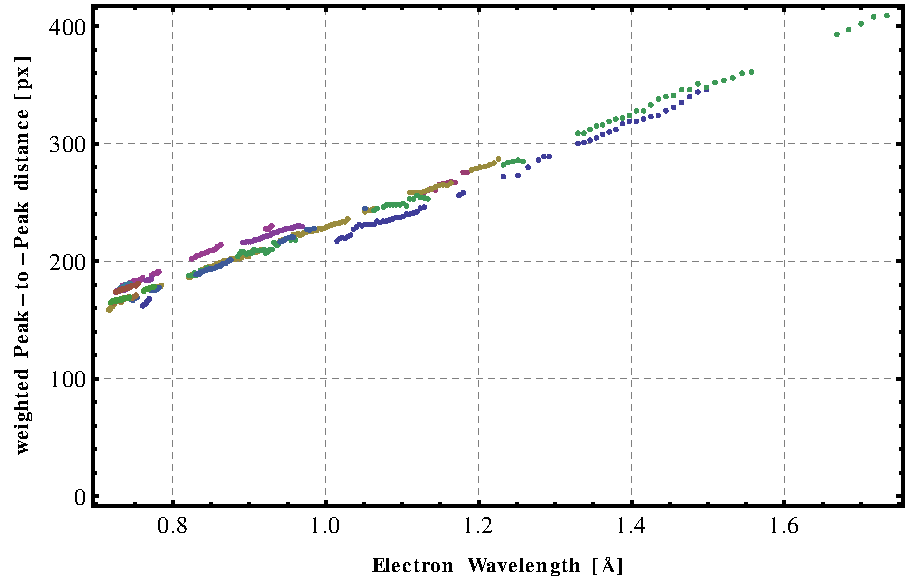
\includegraphics[scale=0.4]{img/allscatter}
\label{fig:allscat}
}
\subfigure[ ]{
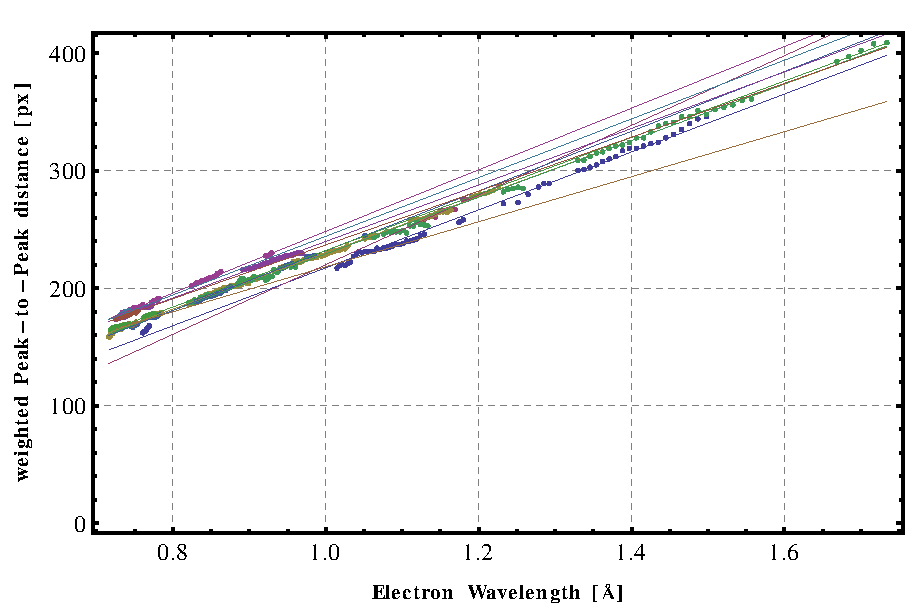
\includegraphics[scale=0.4]{img/allfits}
\label{fig:allfits}
}
\caption{\subref{fig:allscat} shows all peak distance scatter plots combined. \subref{fig:allfits} shows additionally the appropriate fits on top of the distance scatter plots.}
\end{figure}

\subsection{Perpendicular Lattice Constant}

To obtain the perpendicular lattice constant we recorded a intensity spectrum of the (0,0)-peak in the energy range of $40$ to $600\,$eV. The obtained spectrum can be seen in figure~\ref{fig:iv}.

Some of the peaks in that figure are Bragg peaks whereas others are due to other reasons, like inelastic scattering processes.

Since no peaks in figure~\ref{fig:iv} are especially prominent we first obtained the peak positions by fitting them with lorentzians. The third and fourth peak also show small, satellite peaks, so we fitted them once as a whole and once as composite of two single, overlapping peaks. The data for these fits can be found in table~\ref{tab:lorentz}. 

We then went on to make various fits of possible combinations of peaks for various orders to see which peaks would obey the relation
\begin{equation}
E = \left( \frac{12.26\AA}{2a_{\perp}} \right)^{2} n^{2} + V.
\end{equation}
The best fits for this model can be found in table~\ref{tab:ivfitparas}, where the last line can be discarded because the given potential step $V$ is unreasonably big, since it is is more than an order of magnitude greater than the work function of copper, which is about $4.7\,$eV. We see that the other two fits give more reasonable, which is about twice the work function of copper, indicating, that this potential step has another component than the work function. 

The results for $a_{perp}$ we can obtain from the fit parameters in table~\ref{tab:ivfitparas} are  in good agreement with the expected value for the FCC lattice $a_{\perp} = a/2$, which gives a value of $a=1.8\,$\AA~for copper.

\begin{figure}
\centering
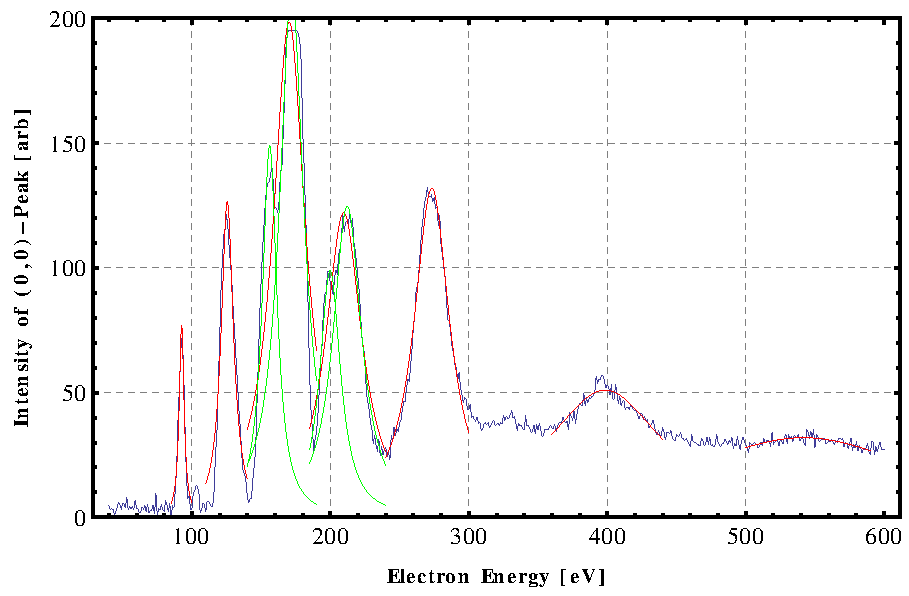
\includegraphics[scale=0.55]{img/iv}
\caption{Intensity spectrum of (0,0)-peak. Single peaks are plotted in red, peaks possibly consisting of two peaks are fitted in green.\label{fig:iv}}
\end{figure}

\begin{table}
\begin{center}
\begin{tabular}{lccc}
\toprule
Peak & A\,[arb]                                        & E$_{0}$\,[eV]                         & $\gamma$\,[eV]                                  \\
\midrule 
1    & $\phantom{0}77.0\phantom{0} \pm 3.0\phantom{0}$ & $\phantom{0}92.50 \pm 0.11$           & $\phantom{00}2.13 \pm 0.16$                     \\
2    & $126.4\phantom{0} \pm 5.4\phantom{0}$           & $125.56 \pm 0.23$                     & $\phantom{00}5.38 \pm 0.34$                     \\
3    & $198.4\phantom{0} \pm 9.3\phantom{0}$           & $170.27 \pm 0.66$                     & $\phantom{0}14.1\phantom{0} \pm 1.1\phantom{0}$ \\
3a   & $148.9\phantom{0} \pm 6.7\phantom{0}$           & $156.18 \pm 0.39$                     & $\phantom{00}6.46 \pm 0.62$                     \\
3b   & $211.0\phantom{0} \pm 7.7\phantom{0}$           & $172.04 \pm 0.39$                     & $\phantom{0}10.67 \pm 0.72$                     \\
4    & $122.1\phantom{0} \pm 3.1\phantom{0}$           & $209.69 \pm 0.39$                     & $\phantom{0}15.82 \pm 0.66$                     \\
4a   & $\phantom{0}98.9\phantom{0} \pm 8.5\phantom{0}$ & $199.9\phantom{0} \pm 2.0\phantom{0}$ & $\phantom{00}9.1\phantom{0} \pm 1.7\phantom{0}$ \\
4b   & $124.7\phantom{0} \pm 1.7\phantom{0}$           & $212.22 \pm 0.23$                     & $\phantom{0}12.46 \pm 0.37$                     \\
5    & $131.9\phantom{0} \pm 1.4\phantom{0}$           & $273.30 \pm 0.16$                     & $\phantom{0}15.68 \pm 0.26$                     \\
6    & $\phantom{0}51.02 \pm 0.49$                     & $398.39 \pm 0.57$                     & $\phantom{0}52.4\phantom{0} \pm 1.6\phantom{0}$ \\
7    & $\phantom{0}31.93 \pm 0.25$                     & $541.6\phantom{0} \pm 1.4\phantom{0}$ & $110.0\phantom{0} \pm 6.6\phantom{0}$           \\  
\bottomrule
\end{tabular}
\end{center}
\par
\caption{Fit parameters for Lorentz fits in figure~\ref{fig:iv}. The peaks are numbered were numbered from left to right. Peaks possibly consisting of two peaks are subdivided with the letters a and b. \label{tab:lorentz}}
\end{table}

\begin{figure}
\centering
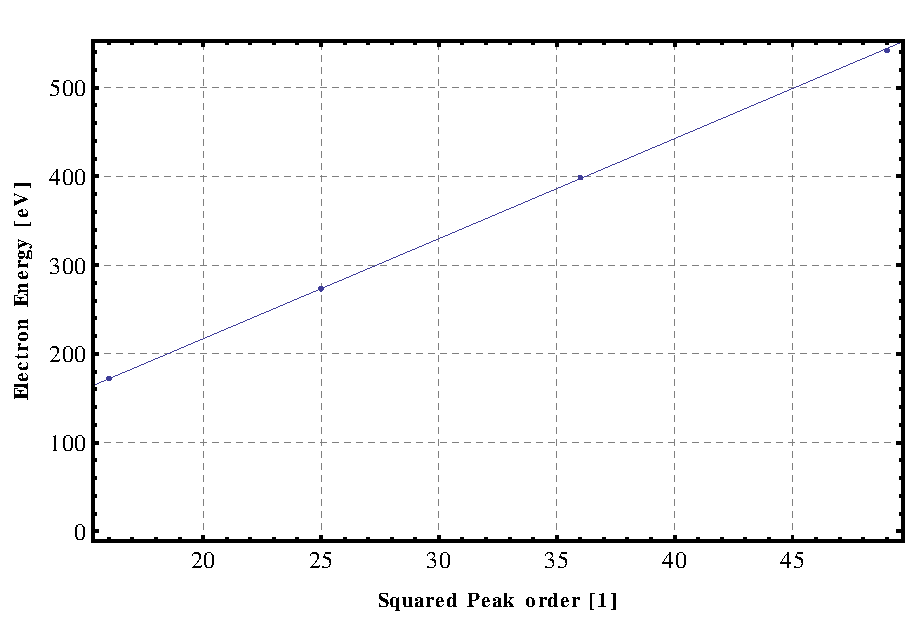
\includegraphics[scale=0.55]{img/ivfit}
\caption{Fit of peak position against squared peak order. \label{fig:ivfit}}
\end{figure}

\begin{table}
\begin{center}
\begin{tabular}{lccccc}
\toprule
Peaks              & Order   & m\,[eV]                      & $U_{0}$\,[eV]               & $R^{2}$  & $a_{\perp}$\,[\AA]  \\
\midrule
3b-5-6-7           & 4-5-6-7 & $11.272 \pm 0.029$           & $-\phantom{0}8.44 \pm 0.73$ & 0.999998 & $1.826 \pm 0.003$ \\
\phantom{b}3-5-6-7 & 4-5-6-7 & $11.324 \pm 0.035$           & $-\phantom{0}9.87 \pm 0.89$ & 0.999997 & $1.819 \pm 0.003$ \\
\phantom{b}3-5-6-7 & 5-6-7-8 & $\phantom{0}9.545 \pm 0.029$ & $-70.2 \pm 1.1\phantom{0}$  & 0.999997 & $1.989 \pm 0.003$ \\
\bottomrule
\end{tabular}
\end{center}
\par
\caption{Fit parameters for peak position vs. order plots. \label{tab:ivfitparas}}
\end{table}


\subsection{Oxygen Superstructure}

\begin{figure}
\centering
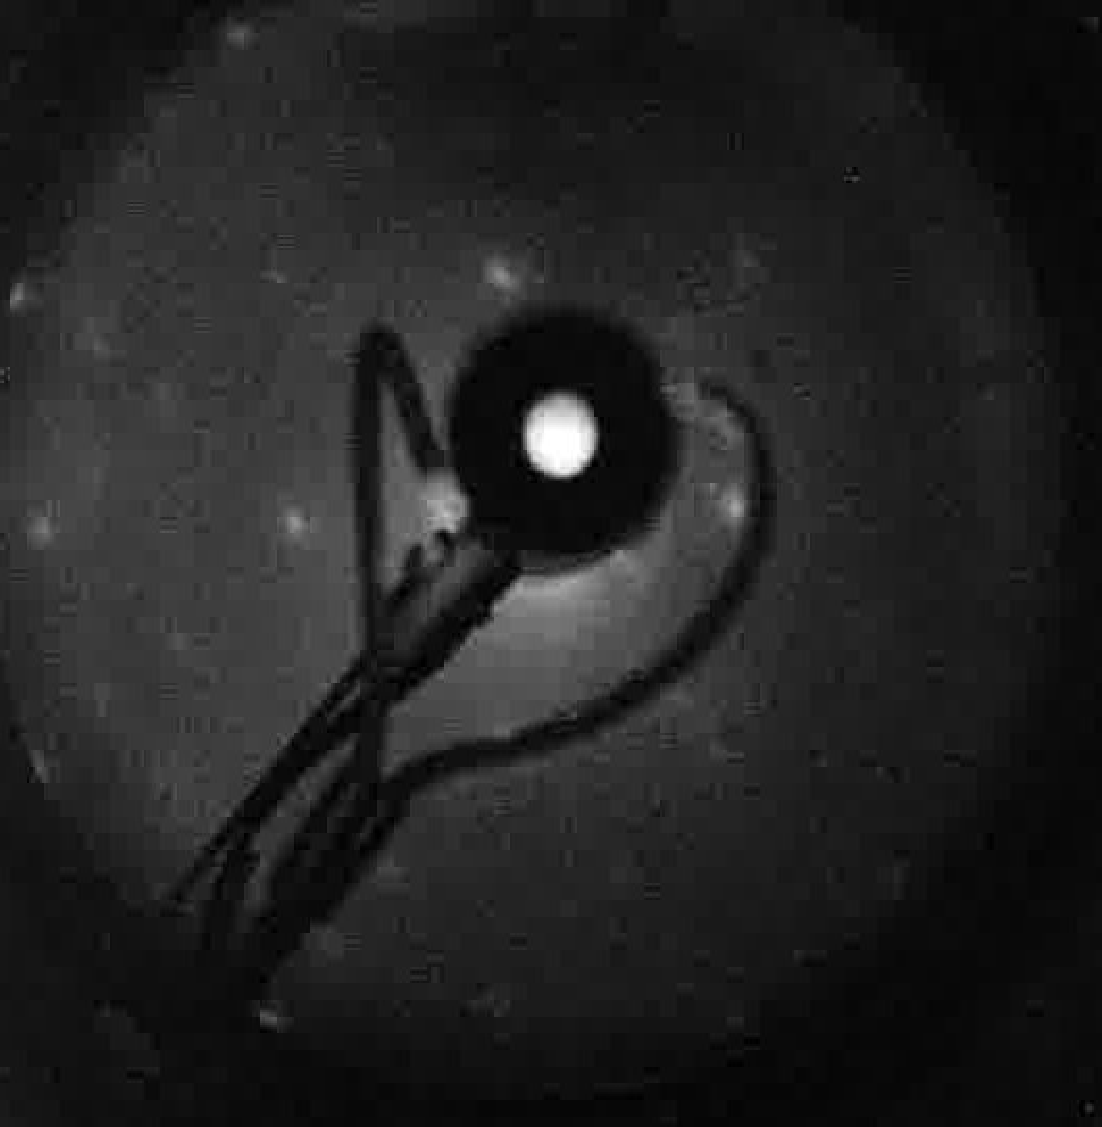
\includegraphics[scale=0.4]{img/img_o2_159eV}
\caption{Image of oxygen superstructure on copper at $159\,$eV. \label{fig:imgo2}}
\end{figure}

Figure~\ref{fig:imgo2} shows an exemplary LEED image at $159\,$eV of the copper sample with the oxygen superstructure. Unfortunately the picture quality is not optimal because of the errors made during the adsorption process, as described earlier. The following descriptions can be seen only qualitatively in figure~\ref{fig:imgo2} but are clearer from viewing the animated scan over the whole energy range.

We can see that additional weaker peaks appear in between the original Cu-(100) peaks. Although weak, we can also see, that between two copper peaks we can find three new peaks, as described in figure~\ref{fig:sup2}. 

Carefully watching the animated scan showed us that the middle peak of the additional three peaks is stronger than the other two peaks, which lead to the realization, that orthogonally to the direction defined by the three additional peaks there are another two peaks. Their superposition makes the middle peak stronger. Thus the observed diffraction pattern can be seen as the superposition of a ($\sqrt{2} \times 2\sqrt{2}$)R$45$\textdegree~and a ($2\sqrt{2} \times \sqrt{2}$)R$45$\textdegree~superstructure. Which makes sense in so far as there is no preferred direction on the copper surface so that domains of each superstructure will form, leading to a superposition of both in the diffraction pattern.

\section{Conclusion}

We successfully determined the lateral lattice constant and perpendicular lattice constant of a copper (100) surface using the method of many images described by Tarasinski and Wölms~\cite{brian}. We obtained the values
\begin{IEEEeqnarray}{rClCrl}
a'        & = & \frac{a}{\sqrt2} & = & (2.43 \pm 0.20)\,\AA \\
a_{\perp} & = & \frac{a}{2}      & = & (1.826 \pm 0.003)\,\AA,
\end{IEEEeqnarray}
which are in agreement with the literary value of $a=3.6\,$\AA for copper~\cite{straumanis}.

We could qualitatively observe the formation of additional peaks due to an oxygen superstructure that was introduced by adsorbing oxygen on the copper surface. We could not validate a preferred direction given as defined by the superstructure ($\sqrt{2} \times 2\sqrt{2}$)R$45$\textdegree~in Woods notation, but observed a superposition of this superstructure with a ($2\sqrt{2} \times \sqrt{2}$)R$45$\textdegree~superstructure. This might be due to errors made during the adsorption process, but is thought to be a general feature, at least in this version of the experiment.

\nocite{skript}
\nocite{henzler}
\nocite{ertl}
\nocite{straumanis}
\nocite{brian}

\bibliographystyle{plainnat}
\bibliography{leed}

\end{document}

% LocalWords:  LEED UHV prevacuum turbomolecular mbar kV mA CCD eV px
% LocalWords:  avi
